

\documentclass{article}


\usepackage[left=1in,right=1in,top=1in,bottom=1in]{geometry}
\usepackage{wrapfig,subfig,graphicx}
\usepackage{latexsym,wasysym,amssymb,marvosym}
\usepackage{framed, color}
\definecolor{shadecolor}{RGB}{205,183,158}
\usepackage{multirow,booktabs}
\usepackage{soul}
\definecolor{navy}{RGB}{0,0,128}
\usepackage{float}
\floatstyle{boxed} 
\restylefloat{figure}

\newcommand{\mcomment}[1]{\textcolor{navy}{#1}}
\newcommand{\bigcheck}{\Large\CrossedBox}
\newcommand{\uncheck}{\Large\HollowBox}


\begin{document}
\renewcommand{\arraystretch}{1.1}


\section*{\LARGE{Douglas Fir-Tan Oak (DFTO)}}

\begin{snugshade}\Large \textbf{General Information} \end{snugshade}

\subsection*{Crosswalks}
PNV Types:
\par Douglas-fir-mcn-tanoak/dry
\par Douglas-fir-mcn-tanoak/moist
\par Douglas-fir-mcn-tanoak/moist\_rocky
\par \hl{Douglas-fir-mcn-canyon live oak/moist}
\par \hl{Douglas-fir-mcn/}
\par \hl{Douglas-fir-mcn/moist}
\par \hl{Douglas-fir-mcn/moist\_rocky}
\par \hl{Douglas-fir-ponderosa pine/moderate}
\par \hl{Douglas-fir-canyon live oak/poison oak/sword fern}
\par \hl{Douglas-fir/moist}
\par \hl{Douglas-fir/moist\_rocky}
\par \hl{canyon live oak}\\
WHR Type: Douglas Fir\\
Wieslander Veg Strings:
\par Pseudotsuga menziesii menziesii--Abies concolor--Lithocarpus densiflorus
\par \hl{Pseudotsuga menziesii menziesii--Abies concolor--Quercus chrysolepis}
\par Pseudotsuga menziesii menziesii--Lithocarpus densiflorus--Arbutus menziesii
\par Pseudotsuga menziesii menziesii--Lithocarpus densiflorus--Quercus chrysolepis
\par \hl{Pseudotsuga menziesii menziesii--Quercus chrysolepis}
\par \hl{Pseudotsuga menziesii menziesii--Quercus chrysolepis}
\par \hl{Pseudotsuga menziesii menziesii--Quercus chrysolepis--Quercus kelloggii}
\par \hl{Pseudotsuga menziesii menziesii--Quercus kelloggii}
\par \hl{Pseudotsuga menziesii menziesii--Quercus kelloggii--Pinus lambertiana--Quercus chrysolepis}
\par \hl{Pseudotsuga menziesii menziesii--Quercus kelloggii--Quercus chrysolepis} \\
Existing Veg Type: \mcomment{Need to discuss with Tahoe folks. I would think that any polygon with Dominant Species Douglas Fir-Tanoak should be classified to DFTO, but most are mixed conifer or montane hardwood/conifer right now.} \\
BpS Model: 0610430 Mediterranean California Mixed Evergreen Forest (shared with Montane Hardwood MHW) \\
\mcomment{Fire return intervals and high/low severity proportions were all calculated based on the BpS model and will need to be adjusted to be specific to DFTO.}


%\paragraph{\large{Vegetation Description}} 
\subsection*{Vegetation Description}

\mcomment{Do we want to use common or scientific names, or both?}
\par This habitat forms a complex mosaic of forest expression due to the geologic, topographic, and successional variation typical within its range. Typical aggregations include a lower overstory of dense, sclerophyllous, broad-leaved evergreen trees (tanoak, Pacific madrone) up to 35 m (114 ft) tall, with an irregular, often open, higher overstory of tall needle-leaved evergreen trees (Douglas-fir) up to 90 m (295 ft). A small number of pole and sapling trees occur throughout stands. On wet sites, shrub layers are well developed, often with 100 percent cover. Cover of the herbaceous layer under the shrubs can be up to 10 percent. At higher elevations, the shrubs disappear and the herb layer is often 100 percent. Diversity of tree size typically increases with stand age, as does tree spacing. Young stands have closely spaced and uniformly distributed trees, whereas older stands show a more patchy stem distribution. Snags and downed logs, an important structural component of this habitat, increase in density or volume with stand age. (WHR)

Deep mesic soils support an overstory of Douglas-fir with a tanoak-dominated understory. (WHR)

In the study area, hardwood tree associates may include Pacific madrone, canyon live oak (\emph{Quercus chrysolepis}), California black oak (\emph{Q. kelloggii}), and California-laurel (\emph{Umbellularia californica}). Potential conifer associates include California white fir (\emph{Abies concolor var. lowiana}), sugar pine (\emph{Pinus lambertiana}), and ponderosa pine (\emph{P. ponderosa var. ponderosa}). (Silvics)

A large variety of shrubs, forbs, grasses, sedges, and ferns are also associated with Douglas Fir-Tanoak. Generally these plants are not abundant once the canopy has closed, but, with tanoak sprouts, often become aggressive on burned or cutover areas. Among the most common shrubs are blueblossom (\emph{Ceanothus thyrsiflorus}), California hazel (\emph{Corylus cornuta} var. \emph{californica}), salal (\emph{Gaultheria shallon}), Pacific bayberry (\emph{Myrica californica}), Pacific rhododendron (\emph{Rhododendron macrophyllum}), flowering currant (\emph{Ribes sanguineum}), thimbleberry (\emph{Rubus parviflorus}), western poison-oak (\emph{Toxicodendron diversilobum}), and California huckleberry (\emph{Vaccinium ovatum}). (Silvics)

Two smaller plants producing woody growth above ground are prince's-pine (\emph{Chimaphila umbellata} var. \emph{occidentalis}) and Oregon grape (\emph{Berberis nervosa}). Among the most important forbs are bull thistle (\emph{Cirsium vulgare}), New Zealand fireweed (\emph{Erechtites arguta}), Australian fireweed (\emph{E. minima}), and western whipplea (\emph{Whipplea modesta}). Common grass species include California brome (\emph{Bromus carinatus}), soft chess (\emph{B. mollis}), California fescue (\emph{Festuca californica}), and California sweetgrass (\emph{Hierochloe occidentalis}). Western swordfern (\emph{Polystichum munitum}) and western bracken (\emph{Pteridium aquilinum} var. \emph{pubescens}) sometimes grow abundantly. Sedges (\emph{Carex} spp.) also are represented in some places. (Silvics)

%\paragraph{\large Distribution}
\subsection*{Distribution}

\paragraph{} Douglas Fir Tanoak is typically found on soils that are deep, well-drained, and loamy, sandy, or gravelly. It grows in valleys, coves, ravines, along streams, and on north slopes. It is found between elevations of 580 and 1220 in (1,900 and 4,000 ft). (Silvics)


%%%%%%%%%%%% DISTURBANCES %%%%%%%%%%%%%%%%
%\newpage
\begin{snugshade}\Large \textbf{Disturbances} \end{snugshade}

\subsection*{Wildfire}

With its flammable leaves and successional position in the understory or subcanopy, tanoak is adapted to catch fire easily. \hl{Despite occurring on wetter soils, the Douglas Fir-Tanoak type experiences more frequent fire than the Douglas Fir type.} In the lower montane zone of the Sierra Nevada where tanoak occurs, the historic fire regime was mixed-severity, dry-season fires of mostly low to moderate severity. Patchy, stand-replacement fires were most common on north-facing slopes and during extended droughts. Most fires occurred in summer or late summer to early fall. (FEIS) Most fires are started by lightning. There is evidence that Native American burning prior to 1850 may have been extensive. (BpS).

Tanoak seedlings and saplings are typically top-killed by even low-severity surface fire. Large trees usually survive moderate-severity fire, bearing fire scars afterward. Even tanoaks with thick bark (1-5 inches (3-10 cm)) typically sustain bole damage from fire. Relative to associated conifers, mature Douglas fir is fairly resistant to surface fires. Crown fires cause extensive mortality. (Silvics)

For mixed evergreen-tanoak, Skinner and Chang report a median FRI of 13, minimum 3, and maximum 41. Van de Water and Safford estimated a mean FRI of 29, median of 13, mean of minimum 15 and mean of maximum 80. Landfire models for this type predict an average FRI of 8. Specifically, replacement fire ranges from 65 to 500 with an average of 333 years, and surface fire ranges from 7 to 15 with an average of 10 years.

Within the cover type, each stage is fairly similarly susceptible to fire. The early development stage is somewhat less susceptible than later stages. Regardless of stage, over 96\% of fires are low mortality events.


\mcomment{The following table reflects BpS setting for Mediterranean California Mixed Evergreen Forest; needs to be adjusted for Douglas Fir-Tanoak.}
\begin{center}
\vspace{.1in}
\begin{tabular}{l|ccccc}
\hline 
\\[-2ex]
 \large Fire Intervals {\small(yrs)} & \textbf{Average} & \textbf{Min} & \textbf{Max} & \textbf{Percent of All Fires} \\
 \hline
 \textbf{High Mortality}	& 75 	& 		& 		& 2.8 	\\
 \textbf{Low Mortality} 	& 8 		& 		& 		& 97.2 	\\
 \textbf{All Fires} 		& 8 		& 	 3	& 41	 	& 		\\
 \multicolumn{5}{l}{\small Numbers from BpS calculations; Skinner and Change.}\\
\hline
\end{tabular}
\end{center}

\subsection*{Other Disturbance}
Other disturbances are not currently modeled, but may, depending on stage affected and mortality levels, reset patches to early development, maintain existing stages, or shift/accelerate succession to a more open stage.

\paragraph{Disease} From seed to maturity, Douglas-fir is subject to serious damage from a variety of agents. Hundreds of fungi, including several types of heart rot fungi, affect Douglas firs. In addition, needle diseases and dwarf mistletoe (\emph{Arceuthobium douglasii}) are widespread. Tanoaks are windfirm and fairly resistant to insect and fungal attacks until fire or other injury damages the bole. Several root- and stem-rotting fungi may infest injured tanoaks. Of these, \emph{Armillaria mellea} generally causes greatest damage.  Tanoak is more susceptible to damage and death from \emph{Phytophthora ramorum}, the fungus-like water mold causing sudden oak death disease, than any other known North American plant. (Silvics)

\paragraph{Insects} Insects are generally not a severe problem for Douglas-fir regeneration. The Douglas-fir tussock moth (\emph{Orgyia pseudotsugata}) and the western spruce budworm (\emph{Choristoneura fumiferana}) are the most important insect enemies of Douglas fir. Both insects attack trees of all ages at periodic intervals, often resulting in severe defoliation of stands. The Douglas-fir beetle (\emph{Dendroctonus pseudotsugae}) is a destructive insect pest in old-growth stands. Several insects feed on tanoak, but their damage is usually minor. (Silvics)

%%%%%%%%%%%%%%%%%%%%%%%%%%VEGETATION CLASSES
\begin{snugshade}\Large \textbf{Vegetation Classes} \end{snugshade}


%%%%%%%		EARLY ALL	%%%%%%%%
\subsection*{Early Development - All (ED)}

\paragraph*{Description} Abundant grasses, forbs, low shrubs, and sparse to moderate cover of trees (primarily \emph{Pseudotsuga menziesii} and \emph{Lithocarpus densiflorus}) seedlings/saplings with an open canopy. This condition is characterized by the diversity of species establishing and reestablishing into an open area created by a stand-replacing disturbance. (CO Model)

Seedling establishment of douglas fir following fire is dependent on the spacing and number of surviving seed trees.  Seedling establishment following large stand-destroying fires may be slow if seed trees are killed over extensive areas. Or, if there are numerous, well-spaced surviving seed trees within the burned area, a new cohort of seedlings can quickly establish. (Silvics) 

Nearly all tan oak burls sprout after fire, and survivorship is high. Canyon live oak, if present, also sprouts readily, and shrubs such as Oregon grape, salal, and rhododendron may be significant. Shrub growth from seed banks, e.g. deer brush (\emph{Ceanothus integerrimus}), can also be high. (BpS)


\paragraph{Succession Transition} The early development stage persists for at least 25 years, after which transition to MDC begins. 

\paragraph{Wildfire Transition} High mortality wildfire recycles the patch through the Early Development stage. Low mortality wildfire is not modeled for this stage. \mcomment{The BpS says there are surface fires; I'm torn about whether to consider them stand replacing or not. I would guess that in this type a surface fire would achieve ''stand replacement" in gaps too small for us to model.}

\noindent\rule{6.5in}{.02pt}


%%%%%%%%% MID DEVELOPMENT CLOSED %%%%%%%%%%%%

\subsection*{Mid Development - Closed (MDC)}

\paragraph{Description}
Sparse ground cover of grasses, forbs, and shrubs; moderate but most likely dense cover of trees (\hl{primarily \emph{Lithocarpus densiflorus}, but also \emph{Pseudotsuga menziesii}}). Other \emph{Quercus} and \emph{Arctostaphylos} species may also be present. (BpS, WHR)

In this stage, hardwoods are dominant (40-100\% canopy cover), but Douglas fir and possibly other conifers are established or establishing under the predominantly tanoak canopy. (BpS, WHR)


\paragraph{Succession Transition} In the absence of disturbance, patches in this class begin transitioning to LDC after 25 years.

\paragraph{Wildfire Transition} High mortality wildfire (2.5\% of fires) recycles the patch through the Early Development stage. Low mortality wildfire (97.5\%) opens up and adds complexity to the stand, but maintains the MDC condition.

\noindent\rule{6.5in}{.02pt}


%%%%%%%%%%%%% LATE DEVELOPMENT CLOSED %%%%%%%%%%%%
\subsection*{Late Development - Closed (LDC)}

%Description
\paragraph{Description} Overstory of large and very large conifers, primarily \emph{Pseudotsuga menziesii}. Canopy cover exceeds 60\%. Sugar pine also occurs. \emph{Lithocarpus densiflorus} is tolerant of both full sun and shade, and usually dominates the subcanopy at this stage. Co-dominance of the upper canopy with Douglas fir is uncommon but possible after extended periods without disturbance. \emph{Quercus} and \emph{Arctostaphylos} species may also be present in the sub canopy. (FEIS, BpS)


\paragraph{Succession Transition} In the absence of high mortality disturbance, this class will maintain.

\paragraph{Wildfire Transition} High mortality wildfire (2.4\% of fires) recycles the patch through the Early Development stage. Low mortality wildfire (97.6\%) usually opens the patch up to MDC, but 25\% of the time it maintains the LDC condition.

%%%%%%%%%%%%%%%%%%%%%%%%%%%%%%%%%%%% DRAFT MODEL %%%%%%%%%%%%%%

\begin{snugshade}\Large \textbf{Draft Models} \end{snugshade}

%\section*{Draft Models}
%\mcomment{Notes on the Figure:}%\\

\begin{figure}
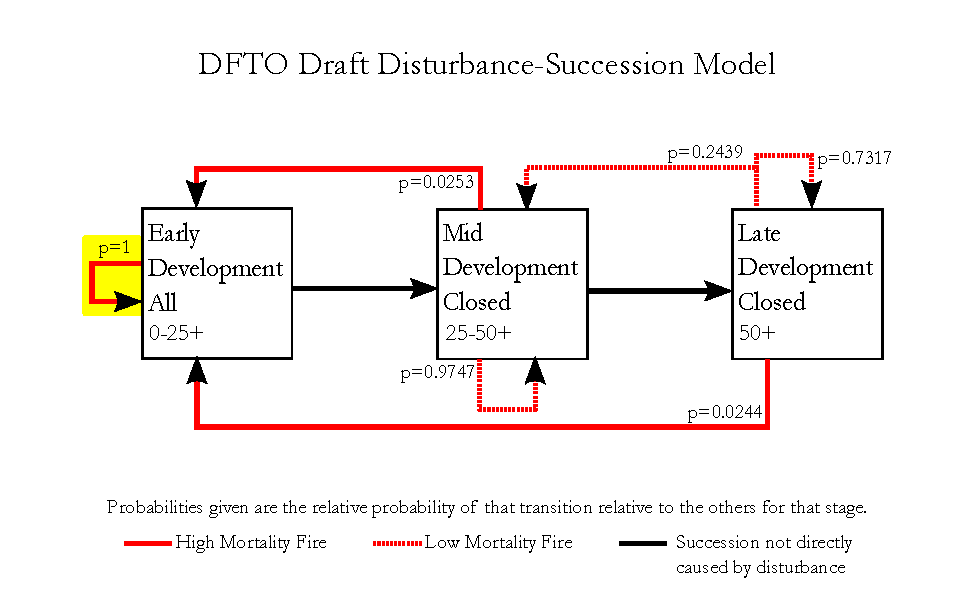
\includegraphics[width=\textwidth]{DFTO_Draft_1.pdf}
\end{figure}


\end{document}











